% Generated by code/scripts/report_figures.py at 2026-10-30T09:20:59Z; do not edit.
% Inputs: artifacts/local/runs/pipeline-e2e-20261030T092022Z/run
\begin{figure}[t]
\centering
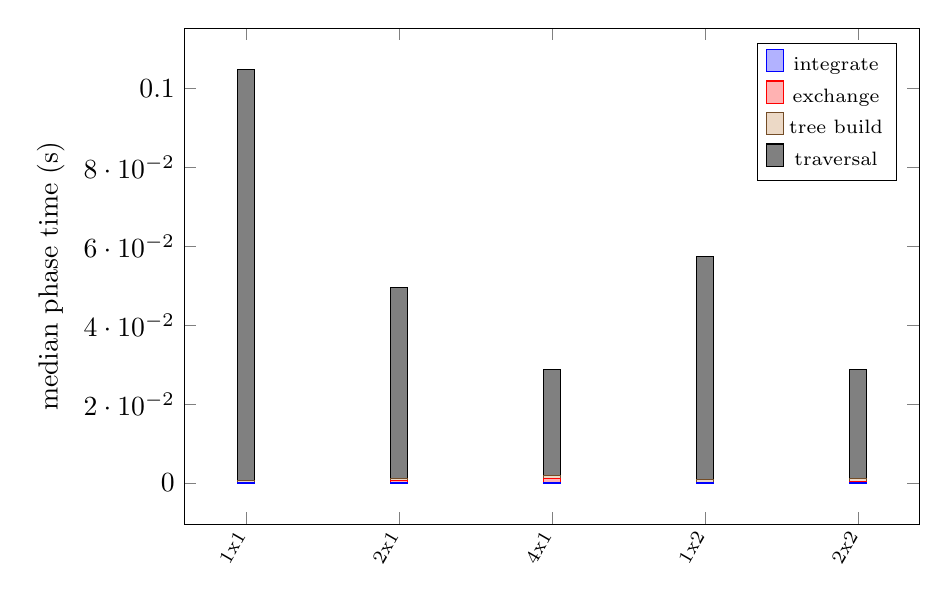
\begin{tikzpicture}
\begin{axis}[ybar stacked, width=0.9\columnwidth, height=0.65\columnwidth, bar width=6pt, symbolic x coords={{1x1},{2x1},{4x1},{1x2},{2x2}}, xtick=data, x tick label style={rotate=60, anchor=east, font=\scriptsize}, ylabel={median phase time (s)}, legend style={font=\scriptsize}, legend pos=north east]
\addplot coordinates {(1x1,5.45e-05) (2x1,2.55e-05) (4x1,1.45e-05) (1x2,9.3e-05) (2x2,2.8e-05)};
\addlegendentry{integrate}
\addplot coordinates {(1x1,2e-06) (2x1,0.000495) (4x1,0.001063) (1x2,2.5e-06) (2x2,0.000453)};
\addlegendentry{exchange}
\addplot coordinates {(1x1,0.000669) (2x1,0.000688) (4x1,0.000769) (1x2,0.0007365) (2x2,0.000687)};
\addlegendentry{tree build}
\addplot coordinates {(1x1,0.1041) (2x1,0.04841) (4x1,0.02691) (1x2,0.05656) (2x2,0.02771)};
\addlegendentry{traversal}
\end{axis}
\end{tikzpicture}
\caption{\textbf{LOCAL PIPELINE TEST, NOT A MEASUREMENT.} Phase breakdown of the strong-scaling hybrid runs (ranks$\times$threads). Each phase is the maximum over ranks, so the stack need not equal the wall time.}
\label{fig:phases}
\end{figure}
